\documentclass{standalone}
\usepackage{tikz}
\usetikzlibrary{positioning}
\usetikzlibrary{calc}

\begin{document}
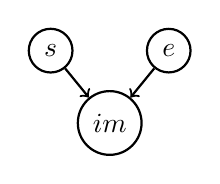
\begin{tikzpicture}[node distance={15mm}, thick, main/.style = {draw, circle}]
    \node[main] (1) {$s$};
    \node[main] (2) [right of=1] {$e$};

    % Calculate midpoint
    \coordinate (midpoint) at ($(1)!0.5!(2)$);

    % Place node 3 above the calculated midpoint (adjust the value as needed)
    \node[main, below=5mm of midpoint] (3) {$im$};

    \draw[->] (1) -- (3);
    \draw[->] (2) -- (3);
\end{tikzpicture}
\end{document}
